\section{HWU Use Case}
A gene is a hereditary unit consisting of a sequence of DNA that occupies a specific location on a chromosome and determines a particular characteristic in an organism. A gene is considered \emph{active} if it is transcribed resulting in one or more RNA products and, following translation, one or more protein products. This phenomenon of transcription and translation is additionally known as gene expression.

Diseases such as cancer, and abnormal features like cleft lips are potentially caused by a change in the genes expressed in an anatomical structure.  In order to investigate such conditions, it is necessary to start by understanding the gene expression in the so-called \emph{normal} (healthy) structures.   EMAGE \cite{emage} is one resource that provides such information to biomedical researchers.  EMAGE, and its developmental mouse \emph{in situ} hybridisation gene expression data was the focus of the HWU use case.

EMAGE's gene expression information is obtained by experimenting on a series of mouse embryos.  Each embryo corresponds to a point in time of the \emph{developmental mouse}: the mouse from conception until birth.  The time window is split into 26 distinct periods called Theiler Stages (TS).  Each stage has its own anatomy, and corresponding anatomy ontology, called EMAP \cite{ema}. 

The initial version of EMAP documented the anatomy as a tree with each structure being \emph{partOf} another, e.g., the digit is \emph{partOf} the paw. Subsequent extensions have resulted in a directed acyclic graph (DAG), yet \emph{partOf} remains the dominant relationship.  %The original tree representation still exists, as a subset of the DAG, and is the favoured visual representation of the anatomy.

The result of an \emph{in situ} hybridization (ISH) experiment is recorded as an image displaying an area of a mouse (from a particular TS) in which some subsections of the mouse are highly coloured, as depicted in Figure \ref{fig:emageResult}. Areas of colour indicate that a gene is expressed in that location. Furthermore, the image provides some indication of the level (strength) of expression: the more intense the colour, the stronger the expression. Results are analysed manually under a microscope. A human expert determines in which anatomical structures the gene is expressed, and at what level of expression. Strength (level) information is described using natural language terms: strong, moderate, weak, possible, detected or not detected. Some of the strength labels are ordered: possible $<$ weak $<$ moderate $<$ strong.  However, `detected' implies any one of weak, moderate or strong.  `Not detected' does not mean the gene is absent, instead it implies the experiment was not sensitive enough to detect the gene.  When a gene is detected, weak, moderate or strong then it is deemed active or \emph{expressed}.  Not detected genes are treated as inactive or \emph{not expressed}.  Genes that have an assignment of `possible' have an unknown level of expression.

Ultimately, when analysing an ISH experiment result (like Figure \ref{fig:emageResult}) the biologist produces a series of \emph{textual annotations}.  Each annotation links a gene, level of expression and anatomical structure at a particular TS.  For example, the gene \emph{Bmp4} is strongly expressed in the future brain from TS15.  The relationships encoded within the textual annotations are what the biomedical researchers are interested in, with common queries including:
\begin{itemize}
\item where is gene $G$ expressed and which other genes are expressed there?
\item which genes are expressed in anatomical structure $S$?
\end{itemize}

\begin{figure}[h] %  figure placement: here, top, bottom, or page
   \centering
   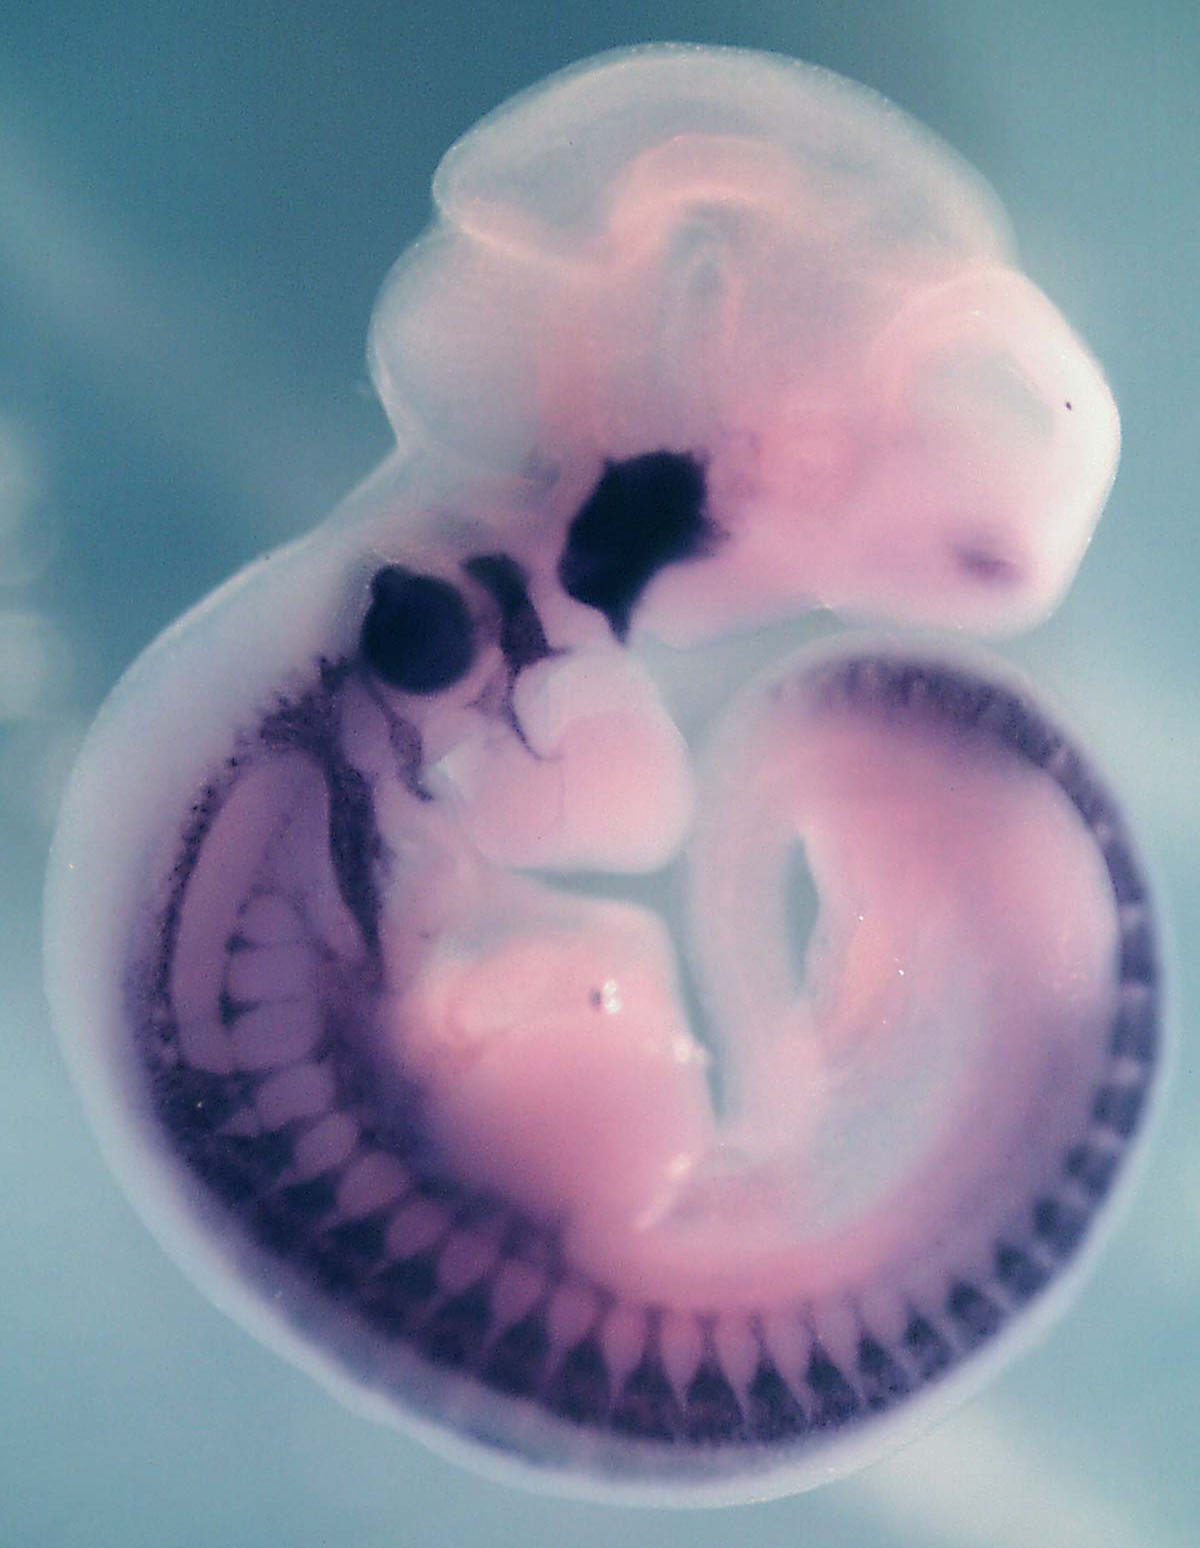
\includegraphics[width=2.5in]{images/emage672} 
   \caption{\textbf{Probably no room for this image?}A sample image of an experimental result from EMAGE (accession ID EMAGE:672).  This image shows a mouse from TS17.  The areas of colour show where the gene \emph{Sox10} is expressed.}
   \label{fig:emageResult}
\end{figure}

%\textbf{This paragraph needs work!} It is the gene - structure relationships that forms the centre of this data set.  Biologists are interested in determining the relationships between genes: in which anatomical structures are genes simultaneously expressed?  Such information helps the researcher determine which experiments to perform in order to investigate abnormal structures or diseases


Another salient feature of the EMAGE repository is the lack of numerical data.  In addition to the textual annotations there is just provenance information: who did what, when and how.  Further distinguishing this use case from those that traditionally deploy BI, is the unhelpfulness of top $k$ queries.  For example, find the top $5$ most expressed genes in the heart?  This query will return the strongly expressed genes that have the most experimental data (i.e., greatest number of experiments indicating that they are strongly expressed in the heart).  However, this merely implies that these genes are very popular.  It is likely that the typical EMAGE user will already know that these genes are active in the heart.  Instead (s)he wishes to discover something new; which are the less renowned genes expressed in the heart?


\begin{thebibliography}{1}
\bibitem{ema} Baldock, R. and Davidson, D. {\em Anatomy for ontologies for bioinformatics: principles and practise} 
chapter: The Edinburgh Mouse Atlas 2008: Springer
 
\bibitem{emage} http://nar.oxfordjournals.org/content/early/2013/11/20/nar.gkt1155 
\end{thebibliography}